\itemhead{p.72 练习 · 第2题（教材p.72）}{XJ-B1-C03-PR-P072-Y1330}
\label{XJ-B1-C03-PR-P072-Y1330}
{\footnotesize 湘教版教材p.72 / PDF第79页 / p.72 练习 / 第2题}
\field{原题}{利用课本中关于水库蓄水量的列表作出由水深确定存水量的函数图象，并根据图象估计出水深为 $7\,\mathrm m$ 和 $18\,\mathrm m$ 时的存水量。
\par\textit{教材p.70被引用的数据：}
\begin{center}\begin{tabular}{c|rrrrrrr}\hline
最大水深 $H/\mathrm m$&5&10&15&20&25&30&35\\
存水量 $Q/(10^4\,\mathrm{m^3})$&20&40&90&160&275&437&650\\\hline
\end{tabular}\end{center}}
\field{参考答案}{在 $H$ 为横轴、$Q$ 为纵轴的坐标系中标出表内7点并用平滑趋势曲线连接。读图参考值分别约为 $28\times10^4$、$132\times10^4$ 立方米（若用相邻数据线性插值）。平滑作图可有差异，答案册示意图读数约25、140，均属估计，不能视为精确唯一值。}
\begin{center}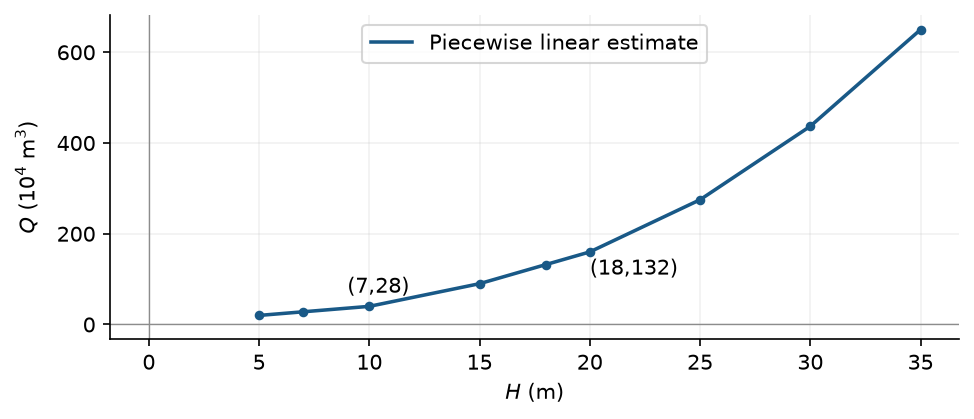
\includegraphics[width=.84\linewidth,height=.38\textheight,keepaspectratio]{figures/C03-PR072-2.png}\end{center}
图为相邻数据的线性插值示例，非唯一的真实库容曲线。\par
\field{核对说明}{读图估计非唯一：表内数据不能唯一确定中间函数值；保留答案册平滑曲线估计25、140，并给线性插值28、132及方法，均不当作精确值。}
{\small \field{关联知识}{F04 函数三种表示法、图象与读数（教材帮p.85、86、93、94 / PDF94、95、102、103）}
\field{方法与易错点}{把关键点与定义域一起标到图上，逐区间读交点和上下关系。 易错：将示意图预测当事实；把两曲线交点收进严格不等式；折线漏端点。}
\field{答案依据}{答案册相关题组：PDF第19页（册内页18）；按当前题库原题逐项重算，不按旧版题号机械对套。}}
